\chapter{\btagging Study}
\label{c:b_tagging_study}

The decay of the \tquark to a \W boson and a \bquark necessitates a thorough understanding of these decay
products in \ttbar events. In particular, methods to identify jets coming from a \bquark, known as \btagging,
are commonly used to increase the efficiency of $\tquark\rightarrow\bquark\W$ signal selection. CMS has
several algorithms for \btagging: TrackCounting (High Efficiency) and TrackCounting (High Purity),
JetBProbability; JetProbability; SoftMuon; SoftMuonByPt; SoftMuonByIP3d; SimpleSecondaryVertex (High
Efficiency); SimpleSecondaryVertex (High Purity); CombinedSecondaryVertex and CombinedSecondaryVetexMVA. These
algorithms produce a discriminator output for each jet which indicates how likely it is to be a \bquark
flavour jet. In all cases, a more positive discriminator value indicates a jet that is more likely to be a
\bquark flavour jet.

The relatively long lifetime (of the order of $10^{-12}\s$) of \bquarks means that they travel a significant
distance (of the order of a few \mm) before decaying. This leads to events with \bjets possessing a secondary
vertex at a distinguishable distance from the primary interaction vertex, as seen in
Figure~\ref{fig:secondary_vertex}. This secondary vertex information, together with track based information
such as the number of tracks in the jet, the invariant mass of the secondary vertex and the impact parameter
significance (described below) of each jet track, is used by the CSV algorithm to produce a discriminator
ranging from 0 to 1, with larger numbers corresponding to a higher probability of a jet being a \bjet. Three
\btagging working points are used in CMS: tight, medium and loose. The medium working point is used in the
different cross sections analysis, which carries a 1~\% mis-tag rate (the rate at which non-\bjets are
mistakenly tagged as \bjets) and approximately 70~\% \btag efficiency.
The tight and loose working points have mis-tag rates of 0.1~\% and 10~\%
respectively~\cite{Chatrchyan:2012jua}.

\begin{figure}[hbtp]
   \centering
     \includegraphics[width=0.8\textwidth]{Chapters/04_Analysis/04a_BTags/Images/b_tagging_graphic}\\
     \caption[Graphical representation of a secondary vertex.]{Graphical representation of an
     interaction originating at the primary vertex producing three jets, one of which is a \bjet with a
     secondary vertex~\cite{d0_fnal}.}
     \label{fig:secondary_vertex}
\end{figure}

\section{Observables used in \btagging algorithms}
\label{s:observables_used_in_btagging_algorithms}

The impact parameter (IP) of a track is defined as the distance between the track and the vertex at the point
of closest approach~\cite{CMS-PAS-BTV-09-001}. Figure~\ref{fig:impact_parameter} shows a schematic
representation of the impact parameter for one single track. The IP measurement can be made in either the
plane transverse to the beam line, or in three dimensions. The impact parameter significance
(IP/$\sigma_{IP}$) is often used instead as an input to \btagging algorithms to allow for the experimental
resolution, due to the fact that the uncertainty on the IP value alone can be as large as the IP itself. The
IP significance distribution of light jets ($\cPqu$, $\cPqd$, $\cPqs$) and gluon jets form a Gaussian
distribution about a mean of zero and width of one, with a slightly extended tail due to tracks from particles
in the jet with long lifetimes. The equivalent distribution for \cjets and \bjets show an asymmetric
distribution at positive values due to the long lifetime of B and C hadrons, making the IP significance a
useful parameter to distinguish between light and heavy flavour jets~\cite{CMS-AN-2005-041}.

The signed IP is also used, in which the sign is obtained from the sign of the scalar product of the IP vector
and the jet direction, so that it is positive if the angle between the IP vector and the jet direction is less
than 90$^{\circ}$, and negative if the angle is greater than 90$^{\circ}$. Tracks belonging in a \bjet would
have an IP sign >0, since the jet direction is an estimate of the direction of travel of the B hadron.
However, the sign could be inaccurately calculated in cases with badly reconstructed jet directions or primary
vertices, or badly measured track parameters~\cite{CMS-AN-2005-041}. Another parameter based on track length,
the 3D decay length significance (the ratio of the three dimensional distance between the primary vertex and
the secondary vertex, and the uncertainty on this value) is also used by some \btagging algorithms.

\begin{figure}[hbtp]
   \centering
     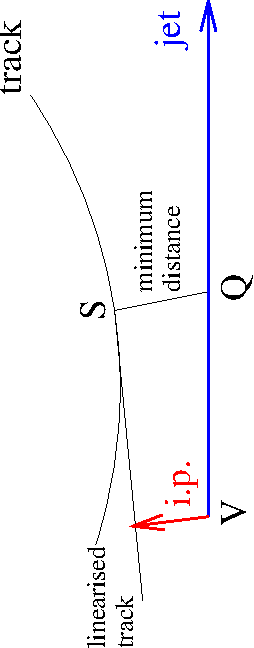
\includegraphics[width=0.8\textwidth]{Chapters/04_Analysis/04a_BTags/Images/impact_parameter}\\
     \caption[Graphical representation of a track impact parameter.]{Graphical representation of a track
     impact parameter~\cite{CMS-PAS-BTV-09-001}.}
     \label{fig:impact_parameter}
\end{figure}

Identification of vertices in CMS consists of two stages: vertex finding and vertex fitting. Vertex finding
deals with the creation of vertex candidates by grouping reconstructed tracks together. Vertex fitting then
deals with obtaining the vertex parameters such as position of the vertex and track parameters, and the
quality of the fit. An adaptive vertex fitter~\cite{0954-3899-34-12-N01} calculates an estimate of the vertex
position and weights tracks based on their compatibility with the vertex. This first fit is constrained to the
interaction region to identify prompt tracks. After removing tracks with weights >0.5, subsequent fits are
carried out to identify potential decay vertices, until no new vertex is identified.

\section{\btagging algorithm descriptions}
\label{s:btagging_algorithm_descriptions}

\subsection*{Track Counting}
\label{ss:track_counting}
The simplest \btagging algorithms available in CMS are the track counting
algorithms~\cite{CMS-PAS-BTV-09-001}, which positively identifies a \bjet if it contains N or more tracks with
IP significance above some theshold value. They function by ordering all good tracks in a jet by order of
decreasing IP significance, with the discriminator being the IP significance of the Nth track. The high
efficiency version of this algorithm uses N=2, i.e. the second track, and the high purity version uses N=3,
i.e. the third track~\cite{CMS-AN-2005-041}.

\subsection*{Jet Probability}
\label{ss:jet_probability}
The ``jet probability'' algorithms~\cite{CMS-PAS-BTV-09-001} produce a discriminator based on the probability that
the set of tracks come from the primary vertex: a high probability would indicate that the jet is not a \bjet,
which would originate at a secondary vertex. These algorithms use all tracks as input and for each track
define an individual probability of coming from the primary vertex. By combining these probabilities, a jet
probability is produced, and the discriminator is the negative log of this confidence
level~\cite{CMS-AN-2005-041}. The ``jet B probability'' variant is based on the four most displaced tracks in
the jet, since the mean number of tracks in a \bjet is approximately 5 and the reconstruction of tracks within
jets has an efficiency of approximately 0.8 in CMS~\cite{CMS-PAS-BTV-09-001}. The ``jet B probability'' in this
case is based on the confidence level that the four most displaced tracks originate from the primary vertex.

\subsection*{Soft Muon}
\label{ss:soft_muon}
The ``soft muon'' algorithms make use of global muons reconstructed in the vicinity of the reconstructed jet,
which may indicate a semi-leptonic decay of B hadrons to a muon~\cite{CMS-AN-2009-085}. Two soft muon
algorithms exist in CMS. The ``soft muon by \pt'' algorithm uses the relative \pt of the muon with respect to
the jet ($p_{T}{rel}$), which is expected to be larger than that for muons in light flavour jets due to the
large \bquark mass~\cite{CMS-AN-2009-085, Ferro:2012tg}. A ``soft muon by IP algorithm'' also exists which
uses the IP significance of positive IP muons. In jets containing more than one muon, the muon with the
highest discriminator is used.

\subsection*{Simple Secondary Vertex}
\label{ss:simple_secondary_vertex}
The simple secondary vertex (SSV) algorithm uses the Adaptive Vertex Fitter to reconstruct the secondary
vertex~\cite{0954-3899-34-12-N01}. The discriminator is calculated based on the 3D decay length significance.
If no secondary vertex is reconstructed, no discriminator is produced, meaning that the efficiency of this
algorithm is limited to the maximum efficiency of secondary vertex reconstruction (approximately
65~\%)~\cite{Chatrchyan:2012jua}. There are two variants of the simple secondary vertex algorithm: the high
efficiency version uses vertices with at least two compatible tracks, whereas the high purity version uses
vertices with at least three tracks. Since this algorithm does not directly use track-based lifetime
parameters, it is less sensitive than other algorithms to tracker misalignment.

\subsection*{Combined Secondary Vertex}
\label{ss:combined_secondary_vertex}
The current CMS recommendation for physics analyses (and therefore the algorithm used in the differential
cross section analysis presented in
Chapters~\ref{c:Differential_Cross_Section:data_simulation_and_selection}-\ref{c:Differential_Cross_Section:systematics_and_results})
is the Combined Secondary Vertex (CSV) algorithm~\cite{Weiser:2006md}. This algorithm reconstructs the event
vertices using the Trimmed Kalman Vertex Finder~\cite{Speer:927395}. This vertex finding algorithm fits tracks
to a primary vertex after removing incompatible tracks and applies cuts to these vertices in order to find a
secondary vertex. The CSV algorithm then combines track-based lifetime parameters, such as IP and flight
distance significance, with secondary vertex information to produce a discriminator. The increased number of
input parameters means that even in cases with no reconstructed secondary vertex a discriminator can be
produced, thereby increasing the maximum efficiency compared to the SSV algorithms~\cite{Chatrchyan:2012jua}.
A variant of this algorithm in which a multi-variate analysis (MVA) is performed using the CMSSW MVA Tools to
produce a discriminator.

\section{Performance Comparison}
\label{s:performance_comparison}

Distributions of the discriminators produced by the above algorithms were created for a \ttbar \MADGRAPH Monte
Carlo simulation sample (/TTJets\_TuneZ2\_7TeV-madgraph-tauola/, produced in the Fall2011 production cycle
using CMSSSW version 44X). A comparison of the discriminator distributions, after normalising to unit area,
for the described algorithms were carried out. Figure~\ref{fig:CSV_discriminators} shows a comparison between
the distributions obtained by the CSV algorithm for the different jets present in the sample: \bjets, light
jets (up, down and strange flavour: \udsjets), gluon jets (\gjets) and charm flavour jets (\cjets). All
distributions were normalised to unity in order to facilitate shape comparision. Equivalent plots for other
algorithms are included in Figure~\ref{fig:all_algorithm_discriminators} in Appendix~\ref{ac:b_tagging_plots}.
In all cases, it can be seen that higher discriminator values were produced for \bjets than for \udsjets,
\gjets and \cjets, as expected.

\begin{figure}[hbtp]
   \centering
     \includegraphics[width=\textwidth]{Chapters/04_Analysis/04a_BTags/Images/CombinedSecondaryVertex_norm_discriminator_combined}\\
     \caption[Discriminator values produced by the Combined Secondary Vertex algorithm after
     normalisation.]{Discriminator values produced by the Combined Secondary Vertex algorithm for all \bjets,
     \cjets, \gjets and \udsjets after normalisation.}
     \label{fig:CSV_discriminators}
\end{figure}

\section{Efficiency}
\label{s:efficiency}

Analyses in CMS make use of \btagging algorithms by placing cuts on the discriminators. The efficiency of a
cut can be defined as the ratio of number of jets passing the selection cut to the total number of jets before
the selection cut. The efficiency was calculated for cut values spanning the whole range of discriminator
values, thereby producing a plot of \btag efficiency as a function of CSV discriminator cut value
(Figure~\ref{fig:CSV_jet_efficiencies}). In practice, the aim is to acheive a high \bjet efficiency and a low
efficiency for all other jet flavours, \ie towards the bottom right of the plot. It can be seen that \udsjets
and \gjets have similar rates of increase in efficiencies with respect to cut value, owing to their similar
discriminator distributions. The \cjet discriminator distribution (Figure~\ref{fig:CSV_discriminators}),
however, has a noticeably different shape. This leads to the undesirable trend of higher \cjet efficiencies
than for \udsjets and \gjets. Equivalent plots for other algorithms can be found in
Figure~\ref{fig:all_algorithm_efficiencies} in Appendix~\ref{ac:b_tagging_plots}.

\begin{figure}[hbtp]
   \centering
     \includegraphics[width=\textwidth]{Chapters/04_Analysis/04a_BTags/Images/CombinedSecondaryVertex_nonBJetEfficiency_v_bJetEfficiency}\\
     \caption[Non \bjet efficiencies as a function of \bjet efficiency for the CSV algorithm.]{Non \bjet
     efficiencies as a function of \bjet efficiency for the CSV algorithm.}
     \label{fig:CSV_jet_efficiencies}
\end{figure}

\section{Algorithm Comparison}
\label{algorithm_comparison}

The performances of the various algorithms can be compared in Figure~\ref{fig:uds_eff_v_b_eff}.

\begin{figure}[hbtp]
   \centering
     \includegraphics[width=\textwidth]{Chapters/04_Analysis/04a_BTags/Images/udsJetEfficiency_v_bJetEfficiency_withLegend_wp}\\
     \caption[udsjet efficiencies as a function of \bjet efficiencies for all algorithms.]{\udsjet
     efficiencies as a function of \bjet efficiencies for all algorithms.}
     %TODO: MAKE PLOT MORE LEGIBLE IF TIME PERMITS
     \label{fig:uds_eff_v_b_eff}
\end{figure}

It can be seen that not all algorithms reach 100~\% \bjet efficiency due to being inherently limited by their
methods. For example, the soft muon algorithms are limited by the muon identification efficiency within \bjets
and also by the branching fraction of B hadrons to muons. The soft muon algorithms all show low maximum \bjet
efficiencies due to the low B hadron semi-leptonic branching ratio to muons of approximately 11~\% (or 20~\%
when further decays are included such as $\cPqb \rightarrow \cPqc \rightarrow l$) \cite{Ferro:2012tg}.
Similarly, the SSV algorithms are limited by the efficiency of reconstructing a secondary vertex in the jet of
approximately 65~\%.

The 2011 and 2012 CMS recommended \btagger is the Combined Secondary Vertex with operating point discriminator
cuts of 0.244 (loose), 0.679 (medium) and 0.898 (tight) corresponding to 10\%, 1\% and 0.1\% light jet
efficiency. These cuts are indicated by the horizontal lines on Figure~\ref{fig:uds_eff_v_b_eff}. It can be
seen that for the tight and medium cuts, the CSV MVA algorithm provides the highest \bjet efficiency and
lowest light jet efficiency, followed closely by the CSV algorithm. The multiple variables that are used as
input allow the CSV algorithm to produce higher efficiencies than the SSV algorithms, while the MVA analysis
variant provides a slightly improved performance. At approximately 3\% light jet efficiency, there is a
convergence of many algorithms that all provide similar performance. At the loose working point also, many of
the algorithms provide similar performance with \bjets, with the ``jet probability'' algorithms marginally
outperforming the CSV algorithms. In early CMSSW versions, it was known that the jet probability algorithm
provided optimal performance, leading to it being recommended for early CMS analyses.
Ultimately, the CSV algorithm provides better performance in CMSSW versions after CMSSW\_2\_X\_Y, at which
point it became the recommended \btagging method.
